\section{Results} \label{results}
% In this section, the results of the test are presented. There are two levels to the test, one where the models are tested on keywords where the same kind of noise is applied, and one where more types of noise are added to the test set. 

\subsection{Testing on BUS and BBL} \label{subsec:test1}
% The different models are tested using a test set created of different sound files where the same kind of noise, as the model is trained on, is added. The results are presented in \Cref{tab:test_noise}, where a subtable for each noise level is presented. 
In this section the accuracy of the trained models when they are tested on new recordings with BUS and BBL noise added. On \Cref{tab:KWT-1_snrmix_busxbbl} the accuracies of the KWT-1 models are presented and on \Cref{fig:KWT-1_snrmix_busxbbl} the accuracies are plotted for a more visual comparison. 
%Here it can be seen that the baseline-supervised have the lowest accyracies and the pretrained-both have the highest.

\begin{table}[H]
    \centering
    \begin{tabular}{@{}llllll@{}}
        \multicolumn{6}{c}{\textbf{KWT-1}}\\
        \toprule
        % &  & & \multicolumn{3}{c}{Data2vec pretraining} \\ \cline{4-6}
        SNR    & \makecell[l]{ Baseline - \\ Supervised } & \makecell[l]{ Baseline - \\ Deta2vec } & \makecell[l]{ Pretrained - \\ Noiseless } & \makecell[l]{ Pretrained - \\ Noisy } & \makecell[l]{ Pretrained - \\ Both } \\ \midrule
        -10  & 0.3459 & 0.3791 & 0.3784 & 0.3827 & 0.3996 \\
        -5   & 0.4805 & 0.5244 & 0.5324 & 0.5537 & 0.5744 \\
        0    & 0.6157 & 0.6641 & 0.6715 & 0.6909 & 0.7107 \\
        5    & 0.6925 & 0.7459 & 0.7558 & 0.7737 & 0.7856 \\
        10   & 0.7335 & 0.7801 & 0.7999 & 0.8086 & 0.8280 \\
        15   & 0.7617 & 0.8120 & 0.8172 & 0.8294 & 0.8509 \\
        20   & 0.7634 & 0.8155 & 0.8288 & 0.8383 & 0.8553 \\
        
        \bottomrule
    \end{tabular}
    \caption{Shows the accuracy of the five models trained using KWT-1, when tested on data with BUS and BBL noise added. The first two columns are the baseline test, a supervised and a SSL trained using only noiseless data. The last three are trained using different data in the pretraning, one uses noiseless, the second uses noisy, and the last uses noisy for the student and noiseless for the teacher.}
    \label{tab:KWT-1_snrmix_busxbbl}
\end{table}

\begin{figure}[H]
    \centering
    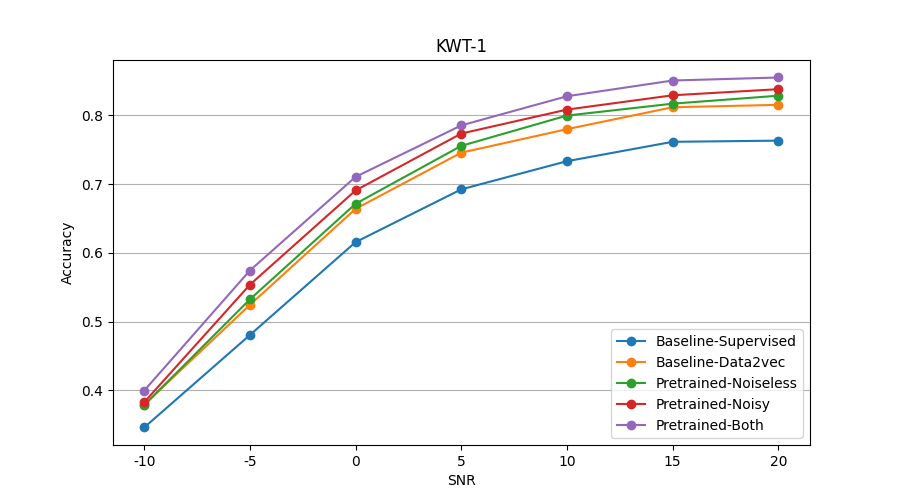
\includegraphics[width=\textwidth]{incl/img/results/kwt1_busxbbl.png}
    \caption{Test plot}
    \label{fig:KWT-1_snrmix_busxbbl}
\end{figure}

Below the accuracies for the KWT-2 models are presented in \Cref{tab:KWT-2_snrmix_busxbbl} the exact accuracies can be read and on \Cref{fig:KWT-2_snrmix_busxbbl} a visual comparition is presented.

\begin{table}[H]
    \centering
    \begin{tabular}{@{}llllll@{}}
        \multicolumn{6}{c}{\textbf{KWT-2}}\\
        \toprule
        % &  & & \multicolumn{3}{c}{Data2vec pretraining} \\ \cline{4-6}
        SNR    & \makecell[l]{ Baseline - \\ Supervised } & \makecell[l]{ Baseline - \\ Deta2vec } & \makecell[l]{ Pretrained - \\ Noiseless } & \makecell[l]{ Pretrained - \\ Noisy } & \makecell[l]{ Pretrained - \\ Both } \\ \midrule
        -10  & 0.3131 & 0.3983 & 0.3888 & 0.4110 & 0.4483 \\
        -5   & 0.4667 & 0.5697 & 0.5728 & 0.5870 & 0.6279 \\
        0    & 0.5958 & 0.7119 & 0.7050 & 0.7294 & 0.7556 \\
        5    & 0.6792 & 0.7974 & 0.7908 & 0.8123 & 0.8349 \\
        10   & 0.7312 & 0.8372 & 0.8320 & 0.8511 & 0.8653 \\
        15   & 0.7536 & 0.8586 & 0.8476 & 0.8673 & 0.8857 \\
        20   & 0.7655 & 0.8632 & 0.8576 & 0.8736 & 0.8871 \\
        
        \bottomrule
    \end{tabular}
    \caption{Shows the accuracy of the five models trained using KWT-2, when tested on data with BUS and BBL noise added. The first two columns are the baseline test, a supervised and a SSL trained using only noiseless data. The last three are trained using different data in the pretraning, one uses noiseless, the second uses noisy, and the last uses noisy for the student and noiseless for the teacher.}
    \label{tab:KWT-2_snrmix_busxbbl}
\end{table}

\begin{figure}[H]
    \centering
    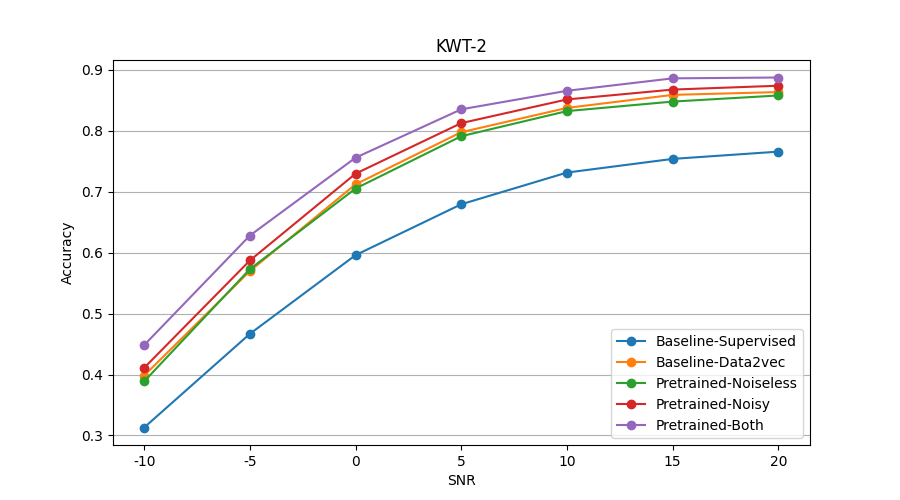
\includegraphics[width=\textwidth]{incl/img/results/kwt2_busxbbl.png}
    \caption{Test plot}
    \label{fig:KWT-2_snrmix_busxbbl}
\end{figure}

Lastly the KWT-3 models, on \Cref{tab:KWT-3_snrmix_busxbbl} the exact accuracies can be found and a more visual comparison on \Cref{fig:KWT-3_snrmix_busxbbl}

\begin{table}[H]
    \centering
    \begin{tabular}{@{}llllll@{}}
        \multicolumn{6}{c}{\textbf{KWT-3}}\\
        \toprule
        % &  & & \multicolumn{3}{c}{Data2vec pretraining} \\ \cline{4-6}
        SNR    & \makecell[l]{ Baseline - \\ Supervised } & \makecell[l]{ Baseline - \\ Deta2vec } & \makecell[l]{ Pretrained - \\ Noiseless } & \makecell[l]{ Pretrained - \\ Noisy } & \makecell[l]{ Pretrained - \\ Both } \\ \midrule
        -10  & 0.2970 & 0.3847 & 0.3602 & 0.3814 & 0.4068 \\
        -5   & 0.4361 & 0.5546 & 0.5083 & 0.5416 & 0.5834 \\
        0    & 0.5738 & 0.6938 & 0.6472 & 0.6794 & 0.7187 \\
        5    & 0.6626 & 0.7832 & 0.7253 & 0.7592 & 0.7965 \\
        10   & 0.7123 & 0.8264 & 0.7695 & 0.7985 & 0.8355 \\
        15   & 0.7474 & 0.8501 & 0.7950 & 0.8201 & 0.8569 \\
        20   & 0.7467 & 0.8598 & 0.7953 & 0.8209 & 0.8575 \\
        
        \bottomrule
    \end{tabular}
    \caption{Shows the accuracy of the five models trained using KWT-3, when tested on data with BUS and BBL noise added. The first two columns are the baseline test, a supervised and a SSL trained using only noiseless data. The last three are trained using different data in the pretraning, one uses noiseless, the second uses noisy, and the last uses noisy for the student and noiseless for the teacher.}
    \label{tab:KWT-3_snrmix_busxbbl}
\end{table}

\begin{figure}[H]
    \centering
    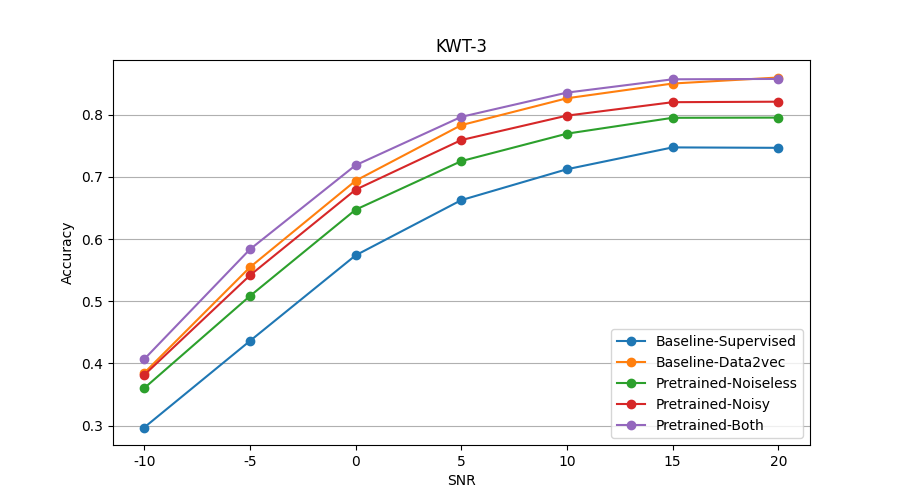
\includegraphics[width=\textwidth]{incl/img/results/kwt3_busxbbl.png}
    \caption{Test plot}
    \label{fig:KWT-3_snrmix_busxbbl}
\end{figure}


\subsection{Testing on BUS, BBL, CAF, and SNN}\label{subsec:test2}
In this section the accuracy of the trained models when they are tested on new recordings with BUS, BBL, CAF, and SNN noise added. On \Cref{tab:KWT-1_snrmix_busxbblxcafxssn} the accuracies of the KWT-1 models are presented and on \Cref{fig:KWT-1_snrmix_busxbblxcafxssn} the accuracies are plotted for a more visual comparison. 
% It can be seen that the baseline-supervised have the lowest accyracies and the pretrained-both have the highest.

\begin{table}[H]
    \centering
    \begin{tabular}{@{}llllll@{}}
        \multicolumn{6}{c}{\textbf{KWT-1}}\\
        \toprule
        % &  & & \multicolumn{3}{c}{Data2vec pretraining} \\ \cline{4-6}
        SNR    & \makecell[l]{ Baseline - \\ Supervised } & \makecell[l]{ Baseline - \\ Deta2vec } & \makecell[l]{ Pretrained - \\ Noiseless } & \makecell[l]{ Pretrained - \\ Noisy } & \makecell[l]{ Pretrained - \\ Both } \\ \midrule
        -10  & 0.2436 & 0.2604 & 0.2541 & 0.2721 & 0.2785 \\
        -5   & 0.3965 & 0.4260 & 0.4319 & 0.4583 & 0.4642 \\
        0    & 0.5443 & 0.5988 & 0.6005 & 0.6304 & 0.6422 \\
        5    & 0.6393 & 0.6941 & 0.7169 & 0.7378 & 0.7523 \\
        10   & 0.7189 & 0.7710 & 0.7809 & 0.7916 & 0.8161 \\
        15   & 0.7544 & 0.7974 & 0.8118 & 0.8234 & 0.8442 \\
        20   & 0.7706 & 0.8215 & 0.8289 & 0.8420 & 0.8608 \\
        
        \bottomrule
    \end{tabular}
    \caption{Shows the accuracy of the five models trained using KWT-1, when tested on data with BUS, BBL, CAF, and SNN noise added. The first two columns are the baseline test, a supervised and a SSL trained using only noiseless data. The last three are trained using different data in the pretraning, one uses noiseless, the second uses noisy, and the last uses noisy for the student and noiseless for the teacher.}
    \label{tab:KWT-1_snrmix_busxbblxcafxssn}
\end{table}

\begin{figure}[H]
    \centering
    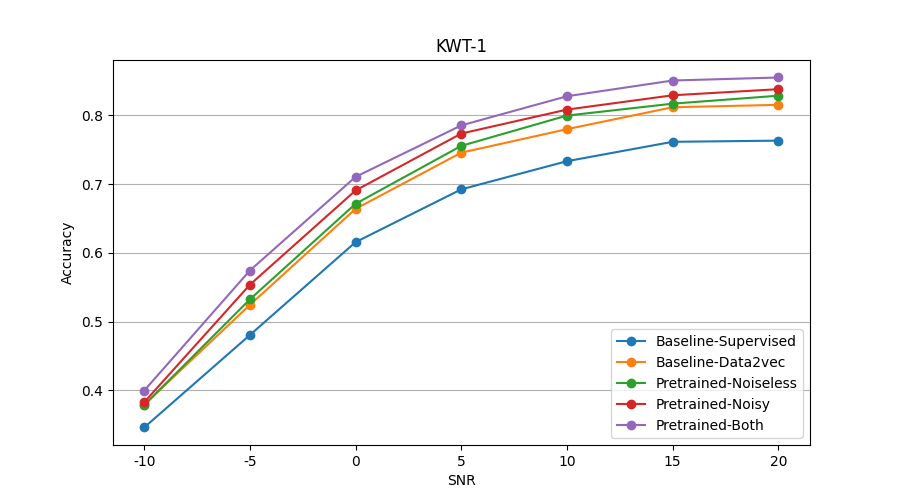
\includegraphics[width=\textwidth]{incl/img/results/kwt1_busxbblxcafxsnn.png}
    \caption{Test plot}
    \label{fig:KWT-1_snrmix_busxbblxcafxssn}
\end{figure}

Below the accuracies for the KWT-2 models are presented in \Cref{tab:KWT-2_snrmix_busxbblxcafxssn} the exact accuracies can be read and on \Cref{fig:KWT-2_snrmix_busxbblxcafxssn} a visual comparition is presented.

\begin{table}[H]
    \centering
    \begin{tabular}{@{}llllll@{}}
        \multicolumn{6}{c}{\textbf{KWT-2}}\\
        \toprule
        % &  & & \multicolumn{3}{c}{Data2vec pretraining} \\ \cline{4-6}
        SNR    & \makecell[l]{ Baseline - \\ Supervised } & \makecell[l]{ Baseline - \\ Deta2vec } & \makecell[l]{ Pretrained - \\ Noiseless } & \makecell[l]{ Pretrained - \\ Noisy } & \makecell[l]{ Pretrained - \\ Both } \\ \midrule
        -10  & 0.2093 & 0.2704 & 0.2748 & 0.2683 & 0.2999 \\
        -5   & 0.3603 & 0.4612 & 0.4612 & 0.4621 & 0.5130 \\
        0    & 0.5149 & 0.6416 & 0.6393 & 0.6622 & 0.6899 \\
        5    & 0.6195 & 0.7605 & 0.7484 & 0.7701 & 0.7957 \\
        10   & 0.6990 & 0.8210 & 0.8158 & 0.8357 & 0.8584 \\
        15   & 0.7408 & 0.8503 & 0.8458 & 0.8632 & 0.8797 \\
        20   & 0.7710 & 0.8668 & 0.8568 & 0.8810 & 0.8898 \\
        
        \bottomrule
    \end{tabular}
    \caption{Shows the accuracy of the five models trained using KWT-2, when tested on data with BUS, BBL, CAF, and SNN noise added. The first two columns are the baseline test, a supervised and a SSL trained using only noiseless data. The last three are trained using different data in the pretraning, one uses noiseless, the second uses noisy, and the last uses noisy for the student and noiseless for the teacher.}
    \label{tab:KWT-2_snrmix_busxbblxcafxssn}
\end{table}

\begin{figure}[H]
    \centering
    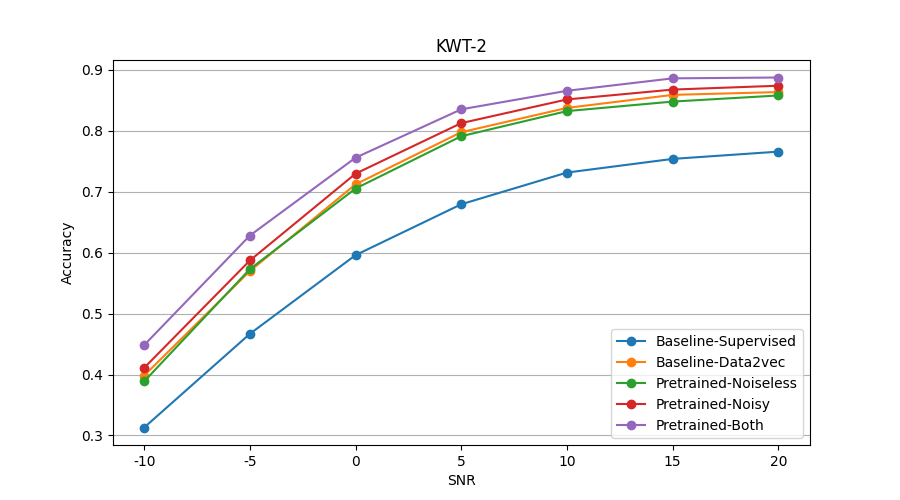
\includegraphics[width=\textwidth]{incl/img/results/kwt2_busxbblxcafxsnn.png}
    \caption{Test plot}
    \label{fig:KWT-2_snrmix_busxbblxcafxssn}
\end{figure}

Lastly the KWT-3 models, on \Cref{tab:KWT-3_snrmix_busxbblxcafxssn} the exact accuracies can be found and a more visual comparison on \Cref{fig:KWT-3_snrmix_busxbblxcafxssn}

\begin{table}[H]
    \centering
    \begin{tabular}{@{}llllll@{}}
        \multicolumn{6}{c}{\textbf{KWT-3}}\\
        \toprule
        % &  & & \multicolumn{3}{c}{Data2vec pretraining} \\ \cline{4-6}
        SNR    & \makecell[l]{ Baseline - \\ Supervised } & \makecell[l]{ Baseline - \\ Deta2vec } & \makecell[l]{ Pretrained - \\ Noiseless } & \makecell[l]{ Pretrained - \\ Noisy } & \makecell[l]{ Pretrained - \\ Both } \\ \midrule
        -10  & 0.2030 & 0.2701 & 0.2427 & 0.2579 & 0.2817 \\
        -5   & 0.3507 & 0.4580 & 0.4065 & 0.4350 & 0.4727 \\
        0    & 0.4961 & 0.6326 & 0.5688 & 0.6115 & 0.6602 \\
        5    & 0.6061 & 0.7437 & 0.6881 & 0.7190 & 0.7587 \\
        10   & 0.6806 & 0.8101 & 0.7500 & 0.7842 & 0.8179 \\
        15   & 0.7256 & 0.8380 & 0.7797 & 0.8069 & 0.8483 \\
        20   & 0.7522 & 0.8532 & 0.8010 & 0.8223 & 0.8635 \\
        
        \bottomrule
    \end{tabular}
    \caption{Shows the accuracy of the five models trained using KWT-3, when tested on data with BUS, BBL, CAF, and SNN noise added. The first two columns are the baseline test, a supervised and a SSL trained using only noiseless data. The last three are trained using different data in the pretraning, one uses noiseless, the second uses noisy, and the last uses noisy for the student and noiseless for the teacher.}
    \label{tab:KWT-3_snrmix_busxbblxcafxssn}
\end{table}

\begin{figure}[H]
    \centering
    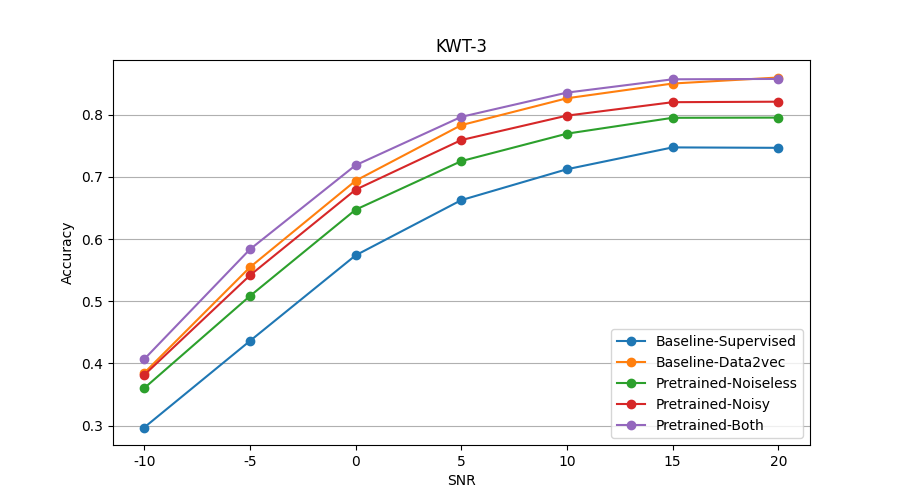
\includegraphics[width=\textwidth]{incl/img/results/kwt3_busxbblxcafxsnn.png}
    \caption{Test plot}
    \label{fig:KWT-3_snrmix_busxbblxcafxssn}
\end{figure}